% =============================================================================
% COPYRIGHT AND DISCLAIMER
% =============================================================================
% This file is provided as a convenience template for competition participants.
% By using it, you accept full responsibility for compliance with all applicable
% copyright, licensing, and usage rules of the Association for Computing
% Machinery (ACM) and of any LaTeX packages you load (including, without
% limitation, the "acmart" document class and related ACM materials).
%
% Consult ACM's official publication, template, and copyright policies before
% using this setup for any purpose other than this competition. Do not assume
% that this template may be reused, redistributed, or submitted elsewhere
% without independently verifying ACM's current rules.
%
% Use of the "acmart" class, the "sigconf" option, or ACM-style formatting in
% this template does NOT mean that this report, this competition, its organizers,
% or any resulting PDF is sponsored, endorsed, affiliated with, or published by
% ACM. ACM trademarks and branding remain the property of ACM.
%
% Template packages live in preamble.tex.
% Citations live in main.bib. Edit this file with your paper content.
% =============================================================================
%
% Report text moved into the organizers' Overleaf template on 17 October 2026
% (overleaf.com/read/vjztpvrnbrdh). This file is the template's main.tex.
% preamble.tex and the first two entries of main.bib are copied from the template.
% The earlier IEEEtran version is kept as report_ieee.tex.

\documentclass[sigconf]{acmart}
% =============================================================================
% Template setup — participants normally do not edit this file.
% Author content belongs in main.tex; citations belong in main.bib.
% \documentclass lives in main.tex so Overleaf does not treat this file as root.
% =============================================================================

% --- Competition / non-ACM-submission friendly rights metadata -------------
\setcopyright{none}
\settopmatter{printacmref=false}
\acmConference[Kaggle Competition]{Filament Segmentation Challenge}{2026}{\href{https://www.kaggle.com/competitions/filament-segmentation-2026}{kaggle.com/competitions/filament-segmentation-2026}}
\acmBooktitle{Competition Report}
\acmDOI{}
\acmISBN{}

% --- Author guidance text --------------------------------------------------
% \guide{...} is gray italic while \guideStyletrue; omitted from the PDF if false.
% Flip the switch in main.tex after % =============================================================================
% Template setup — participants normally do not edit this file.
% Author content belongs in main.tex; citations belong in main.bib.
% \documentclass lives in main.tex so Overleaf does not treat this file as root.
% =============================================================================

% --- Competition / non-ACM-submission friendly rights metadata -------------
\setcopyright{none}
\settopmatter{printacmref=false}
\acmConference[Kaggle Competition]{Filament Segmentation Challenge}{2026}{\href{https://www.kaggle.com/competitions/filament-segmentation-2026}{kaggle.com/competitions/filament-segmentation-2026}}
\acmBooktitle{Competition Report}
\acmDOI{}
\acmISBN{}

% --- Author guidance text --------------------------------------------------
% \guide{...} is gray italic while \guideStyletrue; omitted from the PDF if false.
% Flip the switch in main.tex after % =============================================================================
% Template setup — participants normally do not edit this file.
% Author content belongs in main.tex; citations belong in main.bib.
% \documentclass lives in main.tex so Overleaf does not treat this file as root.
% =============================================================================

% --- Competition / non-ACM-submission friendly rights metadata -------------
\setcopyright{none}
\settopmatter{printacmref=false}
\acmConference[Kaggle Competition]{Filament Segmentation Challenge}{2026}{\href{https://www.kaggle.com/competitions/filament-segmentation-2026}{kaggle.com/competitions/filament-segmentation-2026}}
\acmBooktitle{Competition Report}
\acmDOI{}
\acmISBN{}

% --- Author guidance text --------------------------------------------------
% \guide{...} is gray italic while \guideStyletrue; omitted from the PDF if false.
% Flip the switch in main.tex after \input{preamble}.
%
% Do not use \guide{...} for \email{...}.
\usepackage{xcolor}
\newif\ifguideStyle
\guideStyletrue
\newcommand{\guide}[1]{%
  \ifguideStyle
    {\color{gray!65}\itshape #1}%
  \fi
}

% --- Math ------------------------------------------------------------------
% Do NOT load amssymb (or amsfonts): acmart already loads newtxmath, which
% defines the same symbols (e.g. \Bbbk) and causes a conflict on Overleaf.
% amsmath is already provided by acmart; mathtools extends it.
\usepackage{mathtools}

% --- Figures ---------------------------------------------------------------
% graphicx is already loaded by acmart
\usepackage{subcaption}

% --- Tables ----------------------------------------------------------------
% booktabs is already loaded by acmart
\usepackage{tabularx}
\usepackage{multirow}

% --- Bibliography style is set in main.tex (ACM-Reference-Format) ----------
.
%
% Do not use \guide{...} for \email{...}.
\usepackage{xcolor}
\newif\ifguideStyle
\guideStyletrue
\newcommand{\guide}[1]{%
  \ifguideStyle
    {\color{gray!65}\itshape #1}%
  \fi
}

% --- Math ------------------------------------------------------------------
% Do NOT load amssymb (or amsfonts): acmart already loads newtxmath, which
% defines the same symbols (e.g. \Bbbk) and causes a conflict on Overleaf.
% amsmath is already provided by acmart; mathtools extends it.
\usepackage{mathtools}

% --- Figures ---------------------------------------------------------------
% graphicx is already loaded by acmart
\usepackage{subcaption}

% --- Tables ----------------------------------------------------------------
% booktabs is already loaded by acmart
\usepackage{tabularx}
\usepackage{multirow}

% --- Bibliography style is set in main.tex (ACM-Reference-Format) ----------
.
%
% Do not use \guide{...} for \email{...}.
\usepackage{xcolor}
\newif\ifguideStyle
\guideStyletrue
\newcommand{\guide}[1]{%
  \ifguideStyle
    {\color{gray!65}\itshape #1}%
  \fi
}

% --- Math ------------------------------------------------------------------
% Do NOT load amssymb (or amsfonts): acmart already loads newtxmath, which
% defines the same symbols (e.g. \Bbbk) and causes a conflict on Overleaf.
% amsmath is already provided by acmart; mathtools extends it.
\usepackage{mathtools}

% --- Figures ---------------------------------------------------------------
% graphicx is already loaded by acmart
\usepackage{subcaption}

% --- Tables ----------------------------------------------------------------
% booktabs is already loaded by acmart
\usepackage{tabularx}
\usepackage{multirow}

% --- Bibliography style is set in main.tex (ACM-Reference-Format) ----------

% Added by the authors for the pipeline diagram (Fig. 1).
\usepackage{tikz}
\usetikzlibrary{positioning}

% Guide styling: \guideStyletrue = show gray italic hints; \guideStylefalse = omit them
% \guideStyletrue
\guideStylefalse

\begin{document}

\title{Whole-Disk Context and Metric-Aware Decoding for Solar Filament Instance Segmentation}
\subtitle{A Solution to the Solar Filament Segmentation Challenge 2026} % DO NOT CHANGE


\author{Pragyaan Gaur}
\affiliation{%
  \institution{Department of Physics, National Institute of Technology Agartala}
  \city{Agartala}
  \country{India}
}
\email{pragyaangaur12@gmail.com}

\begin{abstract}
    This report describes our solution to the Solar Filament Segmentation Challenge~2026, a Kaggle competition on automatic segmentation of solar filaments in GONG H-$\alpha$ observations. Two human annotators of the same image agree at a Panoptic Quality (PQ) of only about 0.34, so the labels are noisy and the metric has a low ceiling. Our networks are U-Nets with a ConvNeXt-Tiny encoder that see the whole solar disk at 1536 or 2048 pixels. A small ResNet18 then predicts the IoU that each candidate filament would reach, and we keep a candidate only when this value is high enough to raise PQ. The final step fuses three whole-disk models at the level of single filaments by clustering their overlapping candidates. On 5-fold cross-validation over all 707 training observations, the pipeline reaches a PQ of 0.4571, against 0.4465 for the best single model with a tree-based filter and 0.4242 for our best ensemble of models trained on 512-pixel crops. We also report the ideas that did not help, because several of them are natural first choices for this data.
\end{abstract}

\maketitle

\ifguideStyle
\noindent{\color{gray!65}\itshape
Guide mode is on.}
\par\medskip
\fi

\guide{Please limit your report to four (4) pages, excluding the Acknowledgment and References sections. Throughout this document, please follow these considerations:
\begin{itemize}
    \item Do not alter any text that is currently in black color (except for the emails under authors' name).
    \item Replace all gray text with your own.
    \item When you are done with the report, please replace \texttt{\textbackslash guideStyletrue} with \texttt{\textbackslash guideStylefalse}, to remove any gray text. Alternatively, you can remove any text wrapped in \texttt{\textbackslash guide\{\}},
    \item Be as succinct as possible, and only provide details regarding your own work. For example, there is no need to discuss what solar filaments are, or why filament segmentation matters.
    \item If you must, you can add extra sections.
\end{itemize}}


% ==================================== %
%              INTRODUCTION            %
% ==================================== %
\section{Introduction}
    This report goes over the details of our submitted solution to the Solar Filament Segmentation Challenge~2026 \cite{filament-segmentation-2026}. The challenge, launched on July~10,~2026, is organized by the Earth-Space AI Research (ESAIR) Lab\footnote{\href{https://www.esairlab.com/home}{www.esairlab.com/}}. This challenge utilizes the MAGFiLO dataset for evaluation of the segmentation algorithms \cite{ahmadzadeh2024dataset}. Every filament must be returned as a separate mask, and a prediction only counts when its IoU with an annotated filament is above 0.5. A model must therefore decide where one filament ends and the next begins, and which faint or fragmented structures an annotator would count as a filament at all.

Global context matters more than any other network choice we tested. A model that sees the whole disk at 1536 pixels beats every model trained on crops, and a model that sees the whole disk at only 512 pixels is clearly worse. The choice of which predicted instances to submit is worth as much as a better network, and the labels are noisy enough that the metric rewards fewer, more certain filaments. Models are also best combined at the level of single filaments, because averaging their probability maps softens the edges that the decoder relies on. The code is public at \url{https://github.com/pragyaangaur/NSO-Solar-Filament-Challenge}, and the 15 U-Net checkpoints and 10 CNN heads of the final pipeline are public at \url{https://www.kaggle.com/datasets/pragyaangaur/filament-segmentation-2026-weights}.


% ==================================== %
%              METHODOLOGY             %
% ==================================== %
\section{Methodology}\label{sec:methodology}

Fig.~\ref{fig:pipeline} shows the whole pipeline. We describe each stage below in the order in which we developed it.

% Template item "a graphic illustrating the entire data pipeline": Fig. 1.
\begin{figure}[t]
\centering
\begin{tikzpicture}[
  box/.style={draw, rounded corners=2pt, align=center, font=\scriptsize, text width=2.25cm, minimum height=0.95cm, inner sep=2pt},
  arr/.style={-latex, thick},
  node distance=0.33cm and 0.33cm]
\node[box] (img) {H-$\alpha$ image\\2048$\times$2048, grey};
\node[box, right=of img] (net) {3 U-Nets $\times$ 5 folds\\(1536, 1536 seed 2, 2048), 8-way TTA};
\node[box, right=of net] (map) {15 probability maps, 1024 round trip};
\node[box, below=of map] (dec) {Decode each map: threshold, group, fill holes};
\node[box, left=of dec] (cnn) {ResNet18 head predicts mean IoU per candidate};
\node[box, left=of cnn] (fuse) {Cluster overlapping candidates, keep mean score $>\lambda$};
\draw[arr] (img) -- (net);
\draw[arr] (net) -- (map);
\draw[arr] (map) -- (dec);
\draw[arr] (dec) -- (cnn);
\draw[arr] (cnn) -- (fuse);
\end{tikzpicture}
\caption{The final pipeline on one test image. Each fold model of each of the three U-Nets is a separate fusion member, and the output is one mask per kept cluster.}
\label{fig:pipeline}
\Description{Flow chart of six boxes from the input image through three U-Nets, fifteen probability maps, decoding and the CNN head to the fusion step.}
\end{figure}

\subsection{Data and sampling}

The training set has 707 observations from the GONG network \cite{harvey1996gong}. 411 of them were labelled by one annotator, 145 by two and 151 by three, which gives 1,154 annotated images with about 8,200 filament polygons. An annotated image has 7.1 filaments on average, and the median filament covers about 1,200 pixels of the 2048 by 2048 image. The test set has 180 observations. We use 5-fold cross-validation with folds assigned per observation by a hash of its name, so the annotations of one image never appear in both training and validation. Each fold model is validated on its held-out fold, and all five fold models predict the test set. The quality heads are cross-fitted over five groups of observations in the same way.

\subsection{From crops to the whole disk}

Our first models were U-Nets \cite{ronneberger2015unet} trained on random 512 by 512 crops at full resolution. Their input held the image normalised by the mean brightness of the disk, a contrast-enhanced (CLAHE) copy and the radial position on the disk. The target was the fraction of annotators who marked each pixel. A ResNet34 encoder reached 0.395 out-of-fold (OOF) PQ and a ConvNeXt-Tiny encoder reached 0.409. Crops that cover 1024 pixels and are shrunk to 512 (scale 2) raised PQ to 0.4188, and a weighted average of the scale 1 and scale 2 models reached 0.4242. Shrinking the whole disk to 512 pixels dropped PQ to 0.363, because filaments become only 3 to 5 pixels wide. The network therefore needs both the whole disk and enough resolution, which led to the 1536 model.

\subsection{The 1536 whole-disk model}

The 1536 model is a U-Net with a ConvNeXt-Tiny encoder \cite{liu2022convnext} pretrained on ImageNet-12k and fine-tuned on ImageNet-1k. The decoder has five upsampling stages with 256 down to 16 channels. The input is the single grey channel of the whole image, resized to the training resolution. Besides the filament foreground, the network predicts the boundary of each annotated filament as an auxiliary target that helps it separate filaments that touch. The loss is binary cross-entropy plus soft Dice on the foreground, plus 0.2 times a weighted binary cross-entropy on the boundary.

Each training sample uses the masks of one randomly chosen annotator, so the network sees the full spread of annotation styles. Training runs 30 epochs at 1024 pixels and then 24 epochs at 1536 pixels, with AdamW at a learning rate of $3 \times 10^{-4}$ for the decoder and a five times smaller rate for the encoder. We use a cosine schedule, mixed precision and an exponential moving average (EMA) of the weights. Augmentation uses the eight rotations and flips of the square image and mild photometric changes. One fold trains in about 2 hours on a single NVIDIA T4 GPU.

At test time we average the logits over the eight rotations and flips and resize the map to 2048 pixels. Shrinking this map to 1024 pixels and enlarging it again before decoding raised PQ from 0.4437 to 0.4465. Saving the map at full resolution was worse (0.4394), and a Gaussian blur was worse too. The round trip acts as a mild smoothing that matches the smooth outlines that annotators draw. A second 1536 model uses another random seed and the ImageNet-22k weights of the same encoder.

\subsection{Fine-tuning at 2048 pixels}

To use the full resolution of the image, we continued training each fold's 1536 model for 10 epochs on the whole image at 2048 pixels. Training starts from the EMA weights with a learning rate of $5 \times 10^{-5}$ and one image per step, and two folds take about 1.2 GPU hours. Prediction is the same as for the 1536 model. On folds 0 and 1 (285 observations) the 2048 model scored 0.4516 with the tree head of Section~\ref{sec:decoding} and 0.4556 with the CNN head, against 0.4497 and 0.4547 for the 1536 model. Its own gain is small, and its value shows in fusion. On the same folds, fusing it with the 1536 model gave 0.4580, against 0.4562 for fusing two 1536 seeds.

\subsection{Metric-aware decoding}
\label{sec:decoding}

The probability map is turned into instances in four steps that follow the MAGFiLO annotation protocol. Pixels above a threshold form the foreground. Fragments closer than a few pixels are grouped into one instance, because annotators draw a broken filament as one object. Holes are filled and very small regions are removed. These settings were tuned on OOF maps with the exact PQ.

The decoder produces more candidates than we submit. Our first quality filter computes 14 features per candidate, such as its mean and peak probability, size, elongation and position on the disk. A gradient-boosting regressor (the tree head) predicts the IoU that the candidate would reach with a matching annotation, averaged over the annotators of the image. Following the analysis of the metric in Section~\ref{sec:metric}, we keep a candidate only when this predicted IoU is above a threshold $\lambda$. The best $\lambda$ was between 0.18 and 0.28 in every experiment, close to the theoretical value of PQ/2. The tree head adds between 0.007 and 0.035 PQ to every model we trained.

\subsection{A CNN quality head}

The tree head sees only a few summary numbers per candidate. The CNN head is a ResNet18 \cite{he2016resnet} that sees the candidate itself. For each candidate it takes a 128 by 128 pixel crop with four channels, which are the H-$\alpha$ image, the probability map, the candidate mask and the masks of the other candidates. It regresses the same mean IoU target, and we average two seeds. Its predictions correlate with the true mean IoU at 0.630, against 0.581 for the tree head. On the 1536 model, PQ rises from 0.4465 to 0.4517, and a bootstrap over observations gives a probability of 1.00 that the gain is positive.

The head needs care at test time. Each OOF map comes from one model, while our test maps first averaged the five fold models. Averaged maps have softer edges, with a ratio of in-between to confident pixels of 1.51 on test against 1.23 on OOF, so the head scores test candidates lower. We measured this shift on a labelled stand-in, the average of the OOF maps of two 1536 models. There, the OOF threshold scored 0.4424 and the tree head 0.4404. A threshold that keeps the same share of candidates as on OOF scored 0.4477, close to the best threshold in hindsight (0.4481). The single-model submission therefore uses this share-matched threshold. The same shift affects all our earlier submissions and may explain part of the gap of 0.05 to 0.06 between our local and public scores.

\subsection{Filament-level fusion}

Fusion avoids the shift because it never averages maps. Each member map is decoded into its own candidates, and the CNN head scores each of them. Candidates of different members that overlap with IoU above 0.5 form a cluster. A cluster scores the mean of its members' scores, with zero for a member that has no candidate there, and it is represented by its best-scored candidate. Clusters above the threshold are kept, best first, and a cluster that overlaps a kept one by more than half of the smaller area is skipped.

On test, each fold model is a separate member, so every member map is as sharp as an OOF map. The final pipeline fuses the two 1536 models and the 2048 model, which gives 15 members per test image. At the OOF threshold of 0.20 it keeps 6.46 filaments per image on test against 6.44 on OOF, so no recalibration is needed. The OOF score is flat for thresholds from 0.16 to 0.26.

% Template item "one or more graphics showing a few examples of the segmentations":
% Fig. 2 (annotators and probability map) and Fig. 3 (final fused masks).
\begin{figure*}[t]
\centering
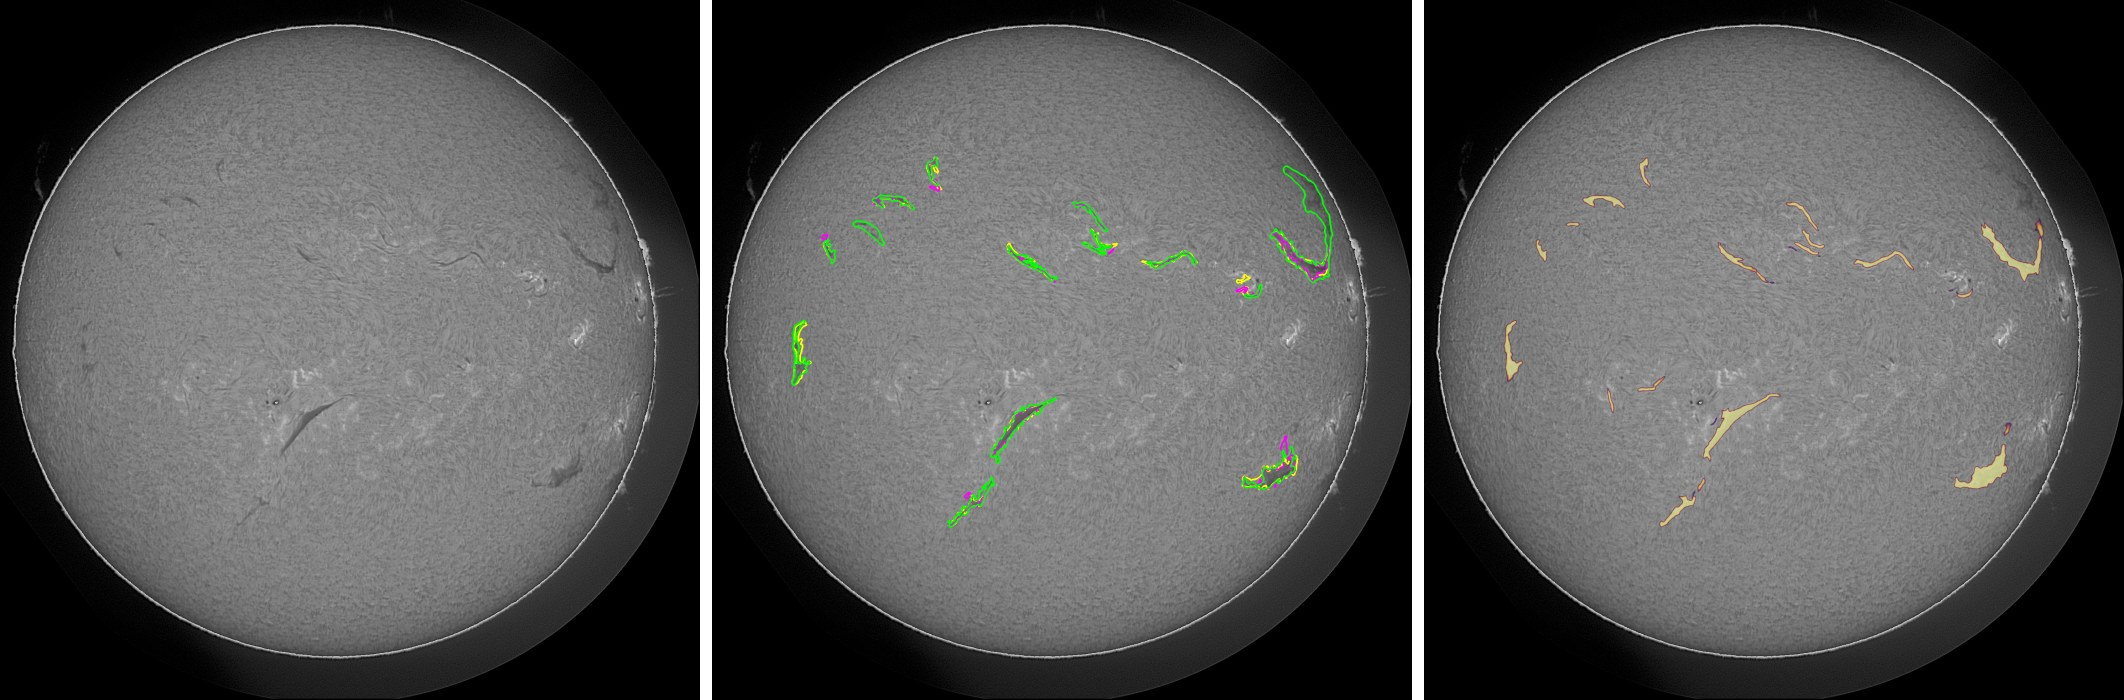
\includegraphics[width=\textwidth]{example.jpg}
\caption{Observation 20150113105034Ch, held out from training (out-of-fold). Left: the GONG H-$\alpha$ image. Middle: the outlines drawn by its three annotators, one colour each (yellow, magenta and green). They agree on the large filaments and differ on the faint and fragmented ones. Right: the probability map of the 1536 whole-disk model, shown where it is above 0.12.}
\label{fig:example}
\Description{Three panels of one solar disk image: the raw image, the annotators' outlines in three colours, and the model's probability map.}
\end{figure*}


% ==================================== %
%              EVALUATION              %
% ==================================== %
\section{Evaluation}\label{sec:evaluation}

\subsection{Metric and evaluation strategy}
\label{sec:metric}

For each annotator of each image, the scorer computes the IoU between every predicted and every annotated mask. A pair with IoU above 0.5 is a true positive, an unmatched prediction is a false positive and an unmatched annotation is a false negative. Counts are pooled over all images, and the score is the Panoptic Quality \cite{kirillov2019panoptic}
\begin{equation}
\mathrm{PQ} = \frac{\sum_{\text{TP}} \mathrm{IoU}}{|\mathrm{TP}| + \frac{1}{2}|\mathrm{FP}| + \frac{1}{2}|\mathrm{FN}|}.
\end{equation}
When masks do not overlap, every true positive removes one false positive and one false negative, and the expression becomes
\begin{equation}
\mathrm{PQ} = \frac{2 \sum_{\text{TP}} \mathrm{IoU}}{N_{\text{pred}} + N_{\text{gt}}}.
\end{equation}
Every submitted instance adds one to the denominator, while it adds to the numerator only if it is matched. An instance therefore raises PQ only when its expected matched IoU is larger than PQ/2, which is the rule behind our decoding.

We scored one annotator's masks against the other annotators of the same observations with the official scorer and found a PQ between 0.32 and 0.34. A model can still score above this value, because it predicts something close to the average annotator, and each annotator is closer to the average than to another single annotator.

All results are OOF PQ over all 707 training observations, computed with the organizers' scorer or with a faster implementation that gives identical numbers. The public leaderboard covers about 90 test images and reports two decimals, so we used it only to check that local gains carried over.

To measure uncertainty we bootstrapped the final pipeline over the 707 observations with 5,000 resamples. Its PQ has a bootstrap standard deviation of 0.0046 and a 95\% confidence interval from 0.4479 to 0.4658. The five folds score 0.4632, 0.4551, 0.4500, 0.4583 and 0.4577, with a mean of 0.4569 and a standard deviation of 0.0048. The six GONG sites range from 0.4495 (L) to 0.4726 (U), and the other four lie between 0.4521 and 0.4623. Differences between rows of Table~\ref{tab:results} under about 0.005 are therefore within this noise. For the gains of the CNN head and the agreement features we also report bootstrap probabilities that the gain is positive.

\subsection{Results}

Table~\ref{tab:results} lists the main steps. Every row uses a quality filter. The CNN head and fusion each add about 0.005 PQ over the step before them, and the 2048 model adds another 0.003. Fusing two 1536 models gave 0.4544, against 0.4477 for decoding their averaged map, so the gain comes from the way the models are combined. The public score was 0.39 for all four submissions that used the CNN head or fusion. This board rounds to two decimals on about 90 images, so it cannot separate differences of this size.

\begin{table}[t]
\centering
\small
\caption{Out-of-fold PQ on 707 training observations and public leaderboard score. The first eight rows use the tree head and the others use the CNN head.}
\label{tab:results}
\begin{tabular}{lcc}
\toprule
Model & OOF PQ & Public \\
\midrule
ResNet34 U-Net, 512 crops & 0.395 & 0.34 \\
ConvNeXt-Tiny U-Net, 512 crops & 0.409 & 0.35 \\
ConvNeXt-Tiny, 1024 crops at 512 & 0.4188 & 0.35 \\
Ensemble of the two crop models & 0.4242 & 0.36 \\
1536 model, 3 flips & 0.4416 & 0.39 \\
1536 model, 8 flips, smoothing & 0.4465 & 0.38 \\
\quad plus agreement features & 0.4480 & \\
Second 1536 model & 0.4398 & \\
\midrule
1536 model, CNN head & 0.4517 & 0.39 \\
Two 1536 models, averaged map & 0.4477 & \\
Two 1536 models, fused & 0.4544 & 0.39 \\
Plus 2048 model, fused (final) & \textbf{0.4571} & 0.39 \\
\quad public notebook rerun$^{\dagger}$ & 0.4568 & \\
\quad plus second-seed 2048$^{*}$ & +0.0005 & \\
\midrule
Human agreement & 0.32--0.34 & \\
\bottomrule
\end{tabular}

\smallskip{\footnotesize $^{*}$Gain over the final fusion on folds 0 and 1 only, within noise, so not used. $^{\dagger}$95\% bootstrap CI 0.4479 to 0.4658.}
\end{table}

\subsection{What did not help}

\emph{More training images from the GONG archive.} We registered neighbouring archive frames to each training image and transferred its labels, which added 3,191 frames. On fold 0 this raised PQ by only 0.005, because the new frames show the same Sun a few minutes apart.

\emph{Low resolution or newer pretraining at the crop scale.} The whole disk at 512 pixels reached 0.363 and received zero weight in every ensemble search. A ConvNeXt-Tiny encoder with DINOv3 weights reached 0.409 at scale 2, below the ImageNet weights (0.4188). Every average of the 1536 model with the crop models scored below the 1536 model alone.

\emph{Growing masks.} Masks are more often too small than too big, yet growing them into weaker pixels or dilating them lowered PQ from 0.419 to between 0.27 and 0.41. Most of the apparent shrinkage is disagreement between annotators. A per-instance re-cut of each mask to its expected best IoU also lowered PQ, from 0.4465 to 0.4271. Splitting candidates along the predicted boundaries lowered PQ at every setting, from 0.4447 to between 0.333 and 0.439.

\emph{Averaging maps of a second seed.} The second 1536 model alone reached 0.4398. Averaging its maps with the first model gave between 0.4417 and 0.4431, below the first model alone, and a pixel-wise maximum gave 0.4473, which is within noise.

\emph{Other 1536 variants.} A ConvNeXt-Small encoder and a target built from annotator consensus each matched the baseline on fold 0. Averaged with the baseline, they raised fold 0 from 0.4469 to 0.4557 together. Over all five folds, ConvNeXt-Small reached 0.4430 alone and 0.4459 averaged with the baseline, below the baseline alone (0.4465), so we stopped the consensus run. A gain of 0.01 on one fold of 139 observations is within fold-to-fold noise. As a third fusion member, ConvNeXt-Small changed PQ by less than 0.001.

\emph{Richer heads.} Agreement features, which count how many other decoder settings produce a nearly identical mask, raised the tree head by only 0.0015 to 0.0023, with bootstrap probabilities of a positive gain between 0.90 and 0.99. We did not keep them once the CNN head was in place. A CNN head trained on the candidates of both 1536 models correlated better with the target (0.652) but gave a fused PQ of 0.4540 against 0.4544.

\subsection{Error analysis}

We classified the errors of the scale 1 and 2 ensemble on half of the training observations. Of the missed filaments, 37\% were not detected at all, and 90\% of these were drawn by only one annotator. 47\% were found with a wrong shape, mostly too small (13\%), merged with a neighbour (11\%) or shifted (11\%). The other 16\% were removed by the quality filter. Of the false predictions, 30\% matched a filament drawn by another annotator of the same image. Filaments near the limb were not a source of error.

For the 1536 model, an oracle that keeps exactly the right candidates scores 0.508, and only 66\% of the annotated filaments are matched by any candidate. Most of the remaining loss is therefore in finding filaments and in choosing among candidates. The shapes of the masks matter less.

\subsection{Reproduction}

We ran the public notebook (\texttt{final/pipeline.ipynb} in our repository) end to end on a Kaggle kernel with two T4 GPUs, from a fresh clone and the public checkpoints, in 1.7 hours. It reproduced an OOF PQ of 0.4568 against 0.4571 in our research run, and the official scorer gives the same value. On the test set, 1,160 of its 1,175 filaments match a submitted filament with IoU above 0.5, with a median IoU of 0.9996. The small difference comes from running inference with other GPU and library versions. The organizers' self-evaluation on OOF gives a segmentation quality (SQ) of 0.6838, a recognition quality (RQ) of 0.6681 and a mean Dice of 0.8090 over matched filaments. In it, 212 annotated filaments touch more than one prediction and 208 predictions touch more than one annotated filament. Fig.~\ref{fig:oof} shows the final masks on two OOF images.

\begin{figure}[t]
\centering
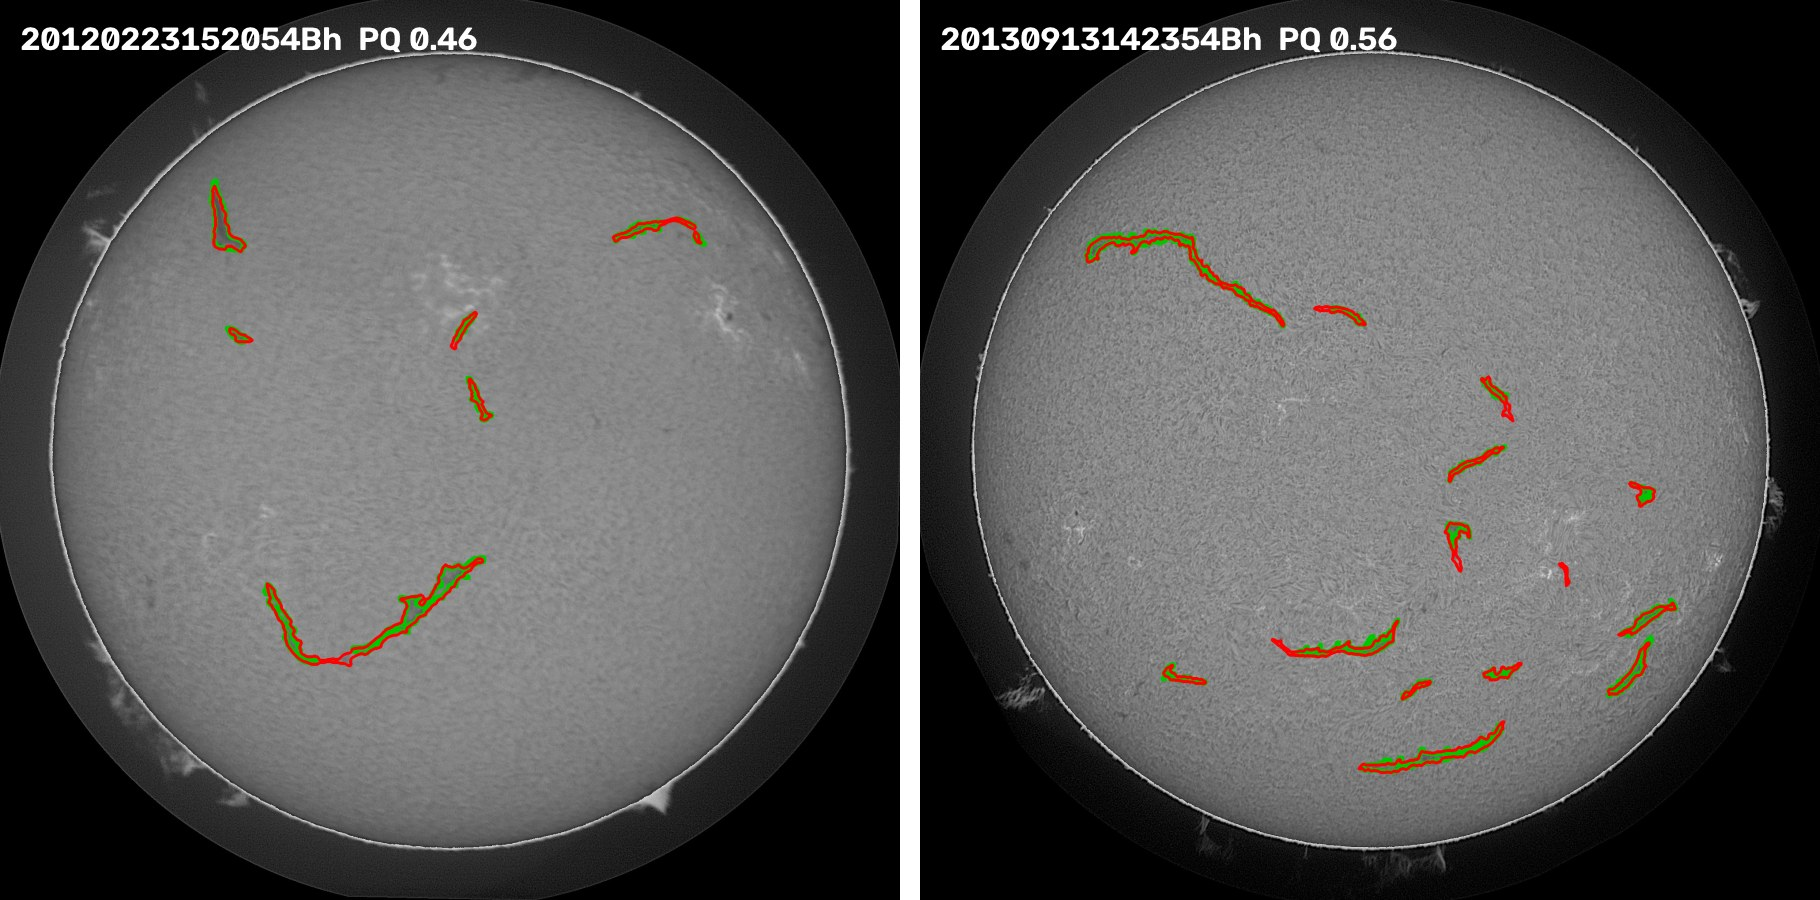
\includegraphics[width=\columnwidth]{examples_oof.jpg}
\caption{Final fused OOF predictions (red) against the first annotator (green) on two observations with five or more annotated filaments. Their per-image PQ of 0.46 and 0.56 lie near the median and the 80th percentile of the training set.}
\label{fig:oof}
\Description{Two solar disk images side by side, each with green annotator outlines and red predicted outlines around the dark filaments.}
\end{figure}

\subsection{Strengths, weaknesses and possible improvements}

The decision of what counts as a filament depends on the whole disk. An annotator sees a long, faint channel as one filament because of its shape across hundreds of pixels, and a crop cuts that shape. With labels this noisy, the metric also rewards caution. The quality filter keeps fewer filaments than a fixed threshold does, and this raises PQ even though it lowers recall.

Our later gains all came from the step after the network. A head that looks at each candidate scores it better than summary features do. Fusion lets each model propose its own candidates and keeps the ones the models agree on, while every member map stays as sharp as during training. The softness shift between single-model and averaged maps is easy to miss, because every averaged ensemble looked worse on OOF while the test maps were averaged by default. A threshold that keeps the same share of candidates is a simple guard against it.

The main weakness is candidate coverage. A third of the annotated filaments are matched by no candidate, and most of them were drawn by only one annotator. The gap between the oracle (0.508) and our selection shows that a better quality head could still gain. The pipeline is also heavy, with 15 U-Nets at 1536 or 2048 pixels and eight-way test-time augmentation for every image.

\section{Conclusion}

Our pipeline fuses three whole-disk U-Nets at 1536 and 2048 pixels at the level of single filaments, and a CNN head keeps only the instances that are expected to raise PQ. It reaches an out-of-fold PQ of 0.4571 on the MAGFiLO training data, against a human agreement of about 0.34 on the same data.


% ==================================== %
%            ACKNOWLEDGMENT            %
% ==================================== %
\section{Acknowledgment}\label{sec:acknowledgment}
    % Do not change
    The organization of the Filament Segmentation Challenge 2026 is partially supported by the U.S. National Science Foundation (NSF) under Grant No. 2209912 and 2433781, directorate for Computer and Information Science and Engineering (CSE), and Office of Advanced Cyberinfrastructure (OAC), and Grant No. 2511630, AST Division Of Astronomical Sciences and MPS Directorate for Mathematical and Physical Sciences.

    The Filament Segmentation Challenge 2026 is sponsored by the U.S. National Science Foundation (NSF) National Solar Observatory (NSO).

    This work utilizes GONG data obtained by the NSO Integrated Synoptic Program, managed by the National Solar Observatory, which is operated by the Association of Universities for Research in Astronomy (AURA), Inc. under a cooperative agreement with the National Science Foundation and with contribution from the National Oceanic and Atmospheric Administration. The GONG network of instruments is hosted by the Big Bear Solar Observatory, High Altitude Observatory, Learmonth Solar Observatory, Udaipur Solar Observatory, Instituto de Astrofísica de Canarias, and Cerro Tololo Interamerican Observatory.

\bibliographystyle{ACM-Reference-Format}
\bibliography{main}

\end{document}
